\documentclass[11pt]{standalone}

\usepackage{ifthen}
\usepackage{tikz} 
\usetikzlibrary{shapes.misc}
\usetikzlibrary{arrows,arrows.meta}
\usetikzlibrary{calc,intersections, patterns, math}

\definecolor{pfeil}{RGB}{168,167,167}
\definecolor{petrol}{RGB}{0, 118, 136}
\definecolor{darkgoldenrod}{RGB}{184, 134, 11}
\colorlet{petrol-lighter}{petrol!40}
\colorlet{darkgoldenrod-lighter}{darkgoldenrod!40}

\begin{document}

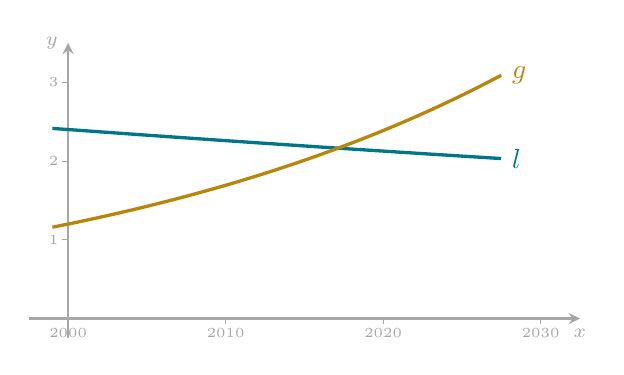
\begin{tikzpicture}[pfeil]

    % \draw[thick, fill=petrol!20, draw=petrol-lighter, rounded corners=2ex, opacity=0.5] (0,0) rectangle ++ (1.5,3.5);
    % \draw[thick, fill=darkgoldenrod!20, draw=darkgoldenrod-lighter, rounded corners=2ex, opacity=0.5] (5,0) rectangle ++ (1.5,3.5);

    \draw[thick, -stealth] (-0.5,0) -- (6.5,0) node[below]{$\scriptstyle x$}; % 2 sind 10 Jahre
	\draw[thick, -stealth] (0,-0.25) -- (0,3.5) node[left]{$\scriptstyle y$};
	
	\draw[very thick,domain=-0.2:5.5, smooth, samples=50, petrol] plot(\x,{2.4*0.994^(5*\x)}) node[right] {$l$};
	\draw[very thick,domain=-0.2:5.5, smooth, samples=50, darkgoldenrod] plot(\x,{1.2*1.035^(5*\x)}) node[right] {$g$};

    \foreach \x in {10,20,...,30}{
        \draw[] (\x/5 ,0) -- ++ (0,-0.075) node[below, yshift=0.75mm] {\tiny 20\x} ;
    }
    \draw[] (0 ,0) -- ++ (0,-0.075) node[below, yshift=0.75mm] {\tiny 2000} ;

    \foreach \x in {1,...,3}{
        \draw[] (0, \x) -- ++ (-0.075,0) node[left, xshift=0.75mm] {\tiny \x} ;
    }


\end{tikzpicture}

\end{document}
